\documentclass{beamer}

\usetheme{Berkeley}

\graphicspath{{../thesis/graphics/}}
\DeclareGraphicsExtensions{.pdf,.jpeg,.jpg,.png}

\usepackage[utf8]{inputenc}
\usepackage{listings}
\usepackage{listing}

\setbeamerfont{frametitle}{family=\rmfamily,series=\bfseries,size={\fontsize{11}{11}}}
\setbeamertemplate{footline}[page number]
\setbeamertemplate{navigation symbols}{} % remove navigation bar

\logo{\includegraphics[width=1.5cm, height=1.5cm]{semiReflectingDragon}}
\author{\textsc{Asger Dam Hoedt}}
\title{\textsc{Efficient Ray Tracing of Dynamic Scenes on the GPU}}

\usepackage{tikz}
\usetikzlibrary{positioning,shadows,arrows}
%Tikz macroes
\tikzset{
  node/.style={rectangle, fill=white, draw, drop shadow},
  visitedNode/.style={rectangle, fill=gray!40, draw, drop shadow},
  leaf/.style={rectangle, rounded corners=1mm, fill=white, draw, drop shadow},
  visitedLeaf/.style={rectangle, rounded corners=1mm, fill=gray!40, draw, drop shadow},
  applyOp/.style={-stealth}
}
\newcommand{\drawTri}[3]{
  \draw[fill=lightgray, drop shadow, rounded corners=0mm] (#1) -- (#2) -- (#3) -- (#1);
}
\newcommand{\drawAabb}[4]{
    \draw[dashed] (#1) -- (#2) -- (#3) -- (#4) -- (#1);
}
\newcommand{\drawRay}[2]{
    \draw[line width=0.5pt, dashed, -stealth] (#1) -- (#2);
}
\newcommand{\drawNode}[4]{
    \draw (#1) -- (#2) -- (#3) -- (#4) -- (#1);
}
\newcommand{\axes}[2]{
  \draw[->] (0,0) -- coordinate (x axis mid) (#1,0);
  \draw[->] (0,0) -- coordinate (y axis mid) (0,#2);
  %ticks
  \foreach \x in {0,2,...,#1}
            \draw (\x,1pt) -- (\x,-3pt)
		    node[anchor=north] {\x};
  \foreach \y in {0,2,...,#2}
     	    \draw (1pt,\y) -- (-3pt,\y) 
     		    node[anchor=east] {\y}; 

}

\newcommand{\scene}{
  % AABB
%  \draw (0,0) -- (10,0) -- (10,8) -- (0,8) -- (0,0);
  
  \axes{11}{9}

  % Tris
  \drawTri{0,2}{2,4}{2,0}
  \draw (1.33,2) node {0};
  \drawTri{2,2}{4,4}{2,4}
  \draw (2.66,3.33) node {1};
  \drawTri{2,2}{4,0}{2,0}
  \draw (2.67,0.67) node {2};

  \drawTri{7,8}{7,4}{9,4}
  \draw (7.67,5.33) node {3};
  \drawTri{9,0}{10,2}{6,3}
  \draw (8.33,1.66) node {4};
  \drawTri{6,3}{6,1}{8,1}
  \draw (6.67,1.67) node {5};
}


\begin{document}

%\tiny

\begin{frame}
  \begin{center}
    \frametitle{Efficient Ray Tracing of Dynamic Scenes on the GPU}
    \footnotesize
    Master's Thesis Exam - April 28, 2011 - Aarhus University
    \vspace*{15pt}\\
    \includegraphics[width=6cm]{semiReflectingDragon}
    \vspace*{20pt}
    \\
    \begin{minipage}{0.4\textwidth}
      \centering
      Asger Dam Hoedt \\ asgerhoedt@gmail.com \\ 20051770
    \end{minipage}
    \begin{minipage}{0.4\textwidth}
      \centering
      Thomas Sangild Sørensen \\ sangild@cs.au.dk \\ Supervisor
    \end{minipage}
  \end{center}
\end{frame}

\section{Introduction}
\begin{frame}
  \frametitle{Motivation}

  \begin{itemize}
  \item Increasing interest in ray tracing for creating photo realistic images.
  \item Usecases include CGI effects in modern films, CAD rendering and lighting
    in games.
  \end{itemize}
\end{frame}

\begin{frame}
  \frametitle{Domain}
  \begin{itemize}
  \item Use KD-tree to accelerate ray tracing.
  \item GPU implementation to utilize the massive computational power of today's
    graphics hardware.
  \end{itemize}
\end{frame}

\begin{frame}
  \frametitle{Goals}
  \begin{itemize}
    \item Minimize the time betwen modifying a scene and presenting visual
      feedback.
    \item Achieve this by examining the relationship between tree quality and
      construction time.
  \end{itemize}
\end{frame}

\section{KD-Trees}
\begin{frame}
  \frametitle{KD-Trees}
  
\end{frame}

\subsection{Example}
\begin{frame}
  \frametitle{Example Scene}
  \begin{minipage}{0.4\textwidth}
    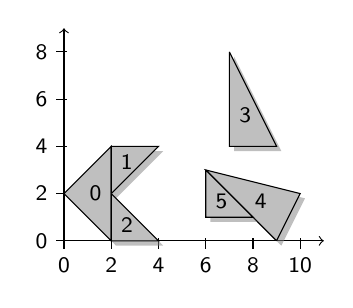
\begin{tikzpicture}[y=0.3cm, x=.3cm,font=\sffamily]
      \footnotesize
      \scene
    \end{tikzpicture}
  \end{minipage}
  \begin{minipage}{0.5\textwidth}
    \centering
    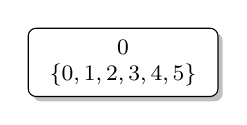
\begin{tikzpicture}[y=0.3cm, x=.3cm,font=\sffamily]
      \footnotesize
      \node [leaf] {$\begin{array}{c}0\\\{0,1,2,3,4,5\}\end{array}$};
    \end{tikzpicture}
  \end{minipage}
\end{frame}

\begin{frame}
  \frametitle{First level split}
  \begin{minipage}{0.4\textwidth}
    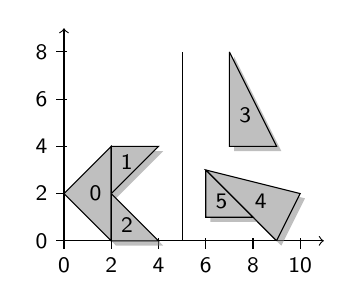
\begin{tikzpicture}[y=0.3cm, x=.3cm,font=\sffamily]
      \footnotesize
      \scene
      
      % splits
      \draw (5,0) -- (5,8);
    \end{tikzpicture}
  \end{minipage}
  \begin{minipage}{0.5\textwidth}
    \centering
    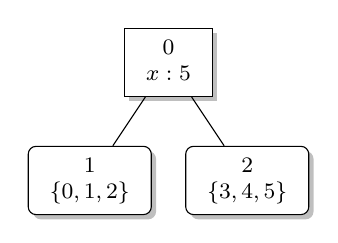
\begin{tikzpicture}[y=0.3cm, x=.3cm,font=\sffamily,
        level 1/.style={sibling distance=20mm}]
      \footnotesize
      \node [node] {$\begin{array}{c}0\\x:5\end{array}$}
        child {node [leaf] {$\begin{array}{c}1\\\{0,1,2\}\end{array}$}}
        child {node [leaf] {$\begin{array}{c}2\\\{3,4,5\}\end{array}$}};
    \end{tikzpicture}
  \end{minipage}
\end{frame}

\begin{frame}
  \frametitle{Second level splits}
  \begin{minipage}{0.4\textwidth}
    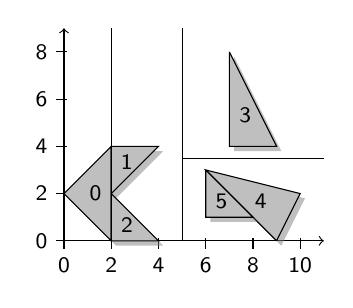
\begin{tikzpicture}[y=0.3cm, x=.3cm,font=\sffamily]
      \footnotesize
      \scene
      
      % splits
      \draw (5,0) -- (5,9);
      \draw (2,0) -- (2,9);
      \draw (5,3.5) -- (11,3.5);
    \end{tikzpicture}
  \end{minipage}
  \begin{minipage}{0.5\textwidth}
    \centering
    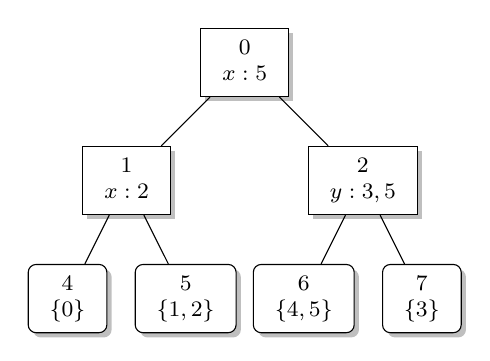
\begin{tikzpicture}[y=0.3cm, x=.3cm,font=\sffamily,level 1/.style={sibling
          distance=30mm}, level 2/.style={sibling distance=15mm}]
      \footnotesize
      \node [node] {$\begin{array}{c}0\\x:5\end{array}$}
        child {node [node] {$\begin{array}{c}1\\x:2\end{array}$}
          child {node [leaf] {$\begin{array}{c}4\\\{0\}\end{array}$}}
          child {node [leaf] {$\begin{array}{c}5\\\{1,2\}\end{array}$}}}
        child {node [node] {$\begin{array}{c}2\\y:3,5\end{array}$}
          child {node [leaf] {$\begin{array}{c}6\\\{4,5\}\end{array}$}}
          child {node [leaf] {$\begin{array}{c}7\\\{3\}\end{array}$}}};
    \end{tikzpicture}
  \end{minipage}
\end{frame}


\subsection{Memory Representation}
\begin{frame}
  \frametitle{Memory Representation}
  \begin{itemize}
  \item How to represent interior nodes and leaf nodes?
  \item How to place the nodes in memory?
  \end{itemize}
\end{frame}

\subsubsection{Node representations}
\begin{frame}[fragile]
  \frametitle{Interior Node Representation}
  An interior node must contain:
  \begin{itemize}
  \item \textit{Split axis} - The axis that an interior node is split
    along.
  \item \textit{Split position} - The position of the splitting plane
    along the split axis.
  \item \textit{Child references} - Information about how to find the
    node's children.
  \end{itemize}

  \begin{lstlisting}[language=C++]
struct KDInterior {
  char axis;
  float splitPosition;
  KDNode *left, *right;
};
  \end{lstlisting}
\end{frame}

\begin{frame}[fragile]
  \frametitle{Leaf Node Representation}
  A leaf node must contain:
  \begin{itemize}
    \item \textit{Associated triangles} - A representation of the triangles
      associated with the leaf node.
  \end{itemize}
  \begin{lstlisting}[language=C++]
struct KDLeaf {
  int triangleIndex, triangleRange;
};
  \end{lstlisting}
\end{frame}

\begin{frame}[fragile]
  \frametitle{Node Representation}
  The complete KDNode is combination of the two node types.
  \begin{lstlisting}[language=C++]
struct KDNode {
  // Contains both node type and axis.
  char nodeType;
  float splitPosition;
  KDNode *left, *right;
  int triangleIndex, triangleRange;
};
  \end{lstlisting}
\end{frame}


\subsubsection{Memory Layout}
\begin{frame}
  \frametitle{Memory Layout}

  \begin{itemize}
  \item The nodes are placed in memory in a linear array.
  
  \item 
    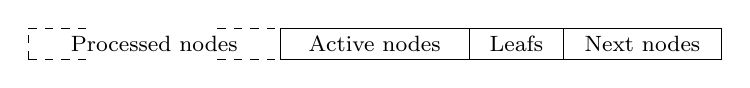
\begin{tikzpicture}[y=0.4cm, x=0.4cm]
      \footnotesize
      
      \draw[dashed] (0,1) -- (2,1);
      \draw[dashed] (0,0) -- (0,1);
      \draw[dashed] (0,0) -- (2,0);
      \draw (4,0.5) node {Processed nodes};
      \draw[dashed] (6,1) -- (8,1);
      \draw[dashed] (6,0) -- (8,0);
      \draw (8,1) -- (8,0);
      
      \draw (8,1) -- (22,1);
      \draw (8,0) -- (22,0);
    
      \draw (11,0.5) node {Active nodes};
      \draw (14,1) -- (14,0);
      
      \draw (15.5,0.5) node {Leafs};
      \draw (17,1) -- (17,0);
      
      \draw (19.5,0.5) node {Next nodes};
      \draw (22,1) -- (22,0);
      
    \end{tikzpicture}
    
  \item This structure allows for coallesced access to the nodes currently being
    processed.
  \end{itemize}
\end{frame}

\subsection{Construction}
\begin{frame}
\end{frame}

\section{Results}
\begin{frame}
\end{frame}

\end{document}
